\documentclass[10pt, openright]{book}

% Load packages, set up document style, and define custom commands
% Document style
\usepackage{geometry}
\usepackage{afterpage}
\usepackage{etoolbox}

% Math notation
\usepackage{amsmath}
\usepackage{amssymb}
\usepackage{amsthm}
\usepackage{bbm}
\usepackage{bm}

% Graphics, colors, and plots
\usepackage{xcolor}
\usepackage{pgfplots}
\usepackage{subcaption}

% Tables and Titles
\usepackage{booktabs}
\usepackage{enumitem}
\usepackage[ruled]{algorithm2e}

% Text, input, and references
\usepackage[swedish, british]{babel}
\usepackage{lmodern}
\usepackage[T1]{fontenc}
\usepackage[utf8]{inputenc}
\usepackage[
    backend=biber,
    style=authoryear, 
    giveninits=false, 
    maxcitenames=2,
    maxbibnames=20,
    uniquename=false,
    uniquelist=false,
    dashed=false
            ]{biblatex}
\usepackage{csquotes}
\usepackage{tocloft}
\usepackage[hidelinks,breaklinks=true]{hyperref}
\usepackage{pdfpages}
\pdfoptionpdfminorversion=7

% Document style
\geometry{
  paperheight=242mm,
  paperwidth=165mm,
  left=22.5mm,
  right=22.5mm,
  top=22.5mm,
  bottom=22.5mm
}
\setlength{\parskip}{2mm}
\setlength{\parindent}{0mm}
\counterwithin*{equation}{chapter}
\setcounter{secnumdepth}{3}

% Plots and figures
\usepgfplotslibrary{groupplots}
\pgfplotsset{compat=1.17}
\usetikzlibrary{shapes,arrows.meta, positioning}

% Change the layout of citations
\DeclareFieldFormat[article,misc]{title}{#1} % Regular font for titles
\DeclareFieldFormat[article,misc]{journaltitle}{\mkbibitalic{#1}} % Italicize journal names
\DeclareFieldFormat[article,misc]{howpublished}{\mkbibitalic{#1}} % Italicize preprint pages
\DeclareNameAlias{sortname}{family-given}
\DeclareNameAlias{default}{family-given}
\renewbibmacro{in:}{}

% Official Stockholm University colors
\definecolor{darkgray}{RGB}{76, 76, 76}
\definecolor{darkblue}{RGB}{0, 47, 95}
\definecolor{green}{RGB}{73, 153, 67}
\definecolor{fireorange}{RGB}{235, 113, 37}
\definecolor{waterblue}{RGB}{155, 178, 206}
\definecolor{red}{RGB}{176, 0, 32}
\definecolor{skyblue}{RGB}{172, 222, 230}
% The remaining colors are not official but match and contrast the former
\definecolor{purple}{RGB}{153, 0, 153}
\definecolor{yellow}{RGB}{255, 204, 0}
\definecolor{teal}{RGB}{0, 128, 128}

% Blank page command for the layout
\newcommand\blankpage{%
    \null
    \thispagestyle{empty}%
    \afterpage{\null\thispagestyle{empty}\newpage}
}

% Redefine some commands to remove page labels
\makeatletter
\renewcommand{\cleardoublepage}{%
  \clearpage
  \if@twoside
    \ifodd\c@page
    \else
      \hbox{}
      \thispagestyle{empty}
      \newpage
    \fi
  \fi
}
\makeatother
\patchcmd{\part}{\thispagestyle{plain}}{\thispagestyle{empty}}{}{}
\renewcommand{\cftaftertoctitle}{\thispagestyle{empty}}

% Full cite command for the list of papers
\newrobustcmd{\fullciteall}[1]{%
  \AtNextCite{\defcounter{maxnames}{4}}%
  \fullcite{#1}%
}


% Notation (edit as you like)
\newcommand{\bg}{\boldsymbol{g}}
\newcommand{\bx}{\mathbf{x}}
\newcommand{\bX}{\mathbf{X}}
\newcommand{\by}{\mathbf{y}}
\newcommand{\bY}{\mathbf{Y}}
\newcommand{\bz}{\mathbf{z}}
\newcommand{\bZ}{\mathbf{Z}}
\newcommand{\bnu}{\boldsymbol{\nu}}
\newcommand{\btheta}{\boldsymbol{\theta}}
\newcommand{\bTheta}{\boldsymbol{\Theta}}
\newcommand{\blambda}{\boldsymbol{\lambda}}
\newcommand{\bLambda}{\boldsymbol{\Lambda}}
\newcommand{\bbeta}{\boldsymbol{\beta}}
\newcommand{\bpsi}{\boldsymbol{\psi}}
\newcommand{\bPsi}{\boldsymbol{\Psi}}
\newcommand{\bphi}{\boldsymbol{\phi}}
\newcommand{\bPhi}{\boldsymbol{\Phi}}
\newcommand{\balpha}{\boldsymbol{\alpha}}
\newcommand{\bAlpha}{\boldsymbol{A}}
\newcommand{\bNu}{\boldsymbol{N}}
\newcommand{\bdelta}{\boldsymbol{\delta}}
\newcommand{\bgamma}{\boldsymbol{\gamma}}
\newcommand{\bGamma}{\boldsymbol{\Gamma}}
\newcommand{\bxi}{\boldsymbol{\xi}}
\newcommand{\bXi}{\boldsymbol{\Xi}}
\newcommand{\argmin}{\operatornamewithlimits{argmin}}
\newcommand{\argmax}{\operatornamewithlimits{argmax}}

% Theorems (edit as you like)
\newtheorem{remark}{Remark}[chapter]

\addbibresource{bibliography.bib}

% Metadata
\title{My PhD Thesis}
\author{Doctor Doktorow}

% Document
\begin{document}

    % Preface stuff
    \frontmatter

    % Note that the abstract here is just a placeholder.
    % The printed thesis will replace the abstract with the "spikblad" but it is included
    % here to keep everything in one place and to include it in the Table of Contents.
    \subsection*{Abstract\addcontentsline{toc}{chapter}{Abstract}\thispagestyle{empty}}
    This thesis presents a groundbreaking series of developments in mathematical theory, solving every known
mathematical problem to date.
Through the integration of advanced computational techniques, innovative algorithms, and a deep understanding
of mathematical principles, this work transcends centuries of mathematical challenges, offering solutions
to problems that have perplexed scholars since the inception of mathematics as a discipline.

Paper I introduces the Universal Solution Algorithm (USA), a computational method that synthesizes existing
mathematical theories with artificial intelligence to find solutions to unsolved problems across various branches
of mathematics, including number theory, algebra, geometry, and calculus.
The USA algorithm demonstrates its efficacy by providing proofs to longstanding conjectures and presenting new
theorems with broad implications.

Paper II focuses on the Complete Theory of Everything (CTE), a framework that unifies all branches of
mathematics under a single, cohesive theory.
This chapter not only solves problems within mathematics but also offers new insights into how mathematics interacts
with physics, biology, and computer science, suggesting a universal language through which all scientific
phenomena can be understood.

Paper III presents the Infinite Complexity Reduction (ICR) method, a technique that simplifies complex
mathematical problems to their most basic elements without losing the essence of the original challenge.
The ICR method has been applied to a range of problems, from the Riemann Hypothesis to P vs NP, demonstrating
unparalleled success in distilling and solving these problems.

Paper IV explores the Multidimensional Proof Generator (MPG), a tool that automates the generation of proofs
for mathematical statements.
This chapter showcases the MPG's ability to produce valid and innovative proofs for theorems that were previously
believed to be unprovable, revolutionizing the way mathematical research is conducted.


        % List of papers
        \chapter*{List of Papers\addcontentsline{toc}{chapter}{List of papers}}
        \thispagestyle{empty}
        \addtocounter{page}{6} % Accounting for left-aligned page and open right for dirt title, title, dedication
        This thesis is based on two papers, numbered I--II, which are included
in the following order.

\begin{enumerate}[label=\Roman*.]
   \item \fullciteall{supervisor2020universal}
   
   \item \fullciteall{researcher2021complete}

   \item \fullciteall{emeritus2023infinite}
   
   \item \fullciteall{doctorow2023multidimensional}

\end{enumerate}

\textbf{Authors' contributions:}
In Paper I, D. Doctorow developed the Universal Solution Algorithm (USA) and wrote the paper.
M. Supervisor was just there for the ride.

In Paper II, D. Doctorow developed the Complete Theory of Everything (CTE) and wrote the paper, as well
as implementing the theory in the \texttt{python} package \texttt{cte}.
P. Researcher was included as an author in order to make the paper more credible, and remains
unclear why E. Colleague was included as an author.

In Paper III, D. Doctorow did not do much, but helped O. Emeritus to write the paper on a computer and was therefore
included as an author.


        % Acknowledgements
        \blankpage
        \chapter*{Acknowledgements}
        \thispagestyle{empty}
        \addcontentsline{toc}{chapter}{Acknowledgements}
        First and foremost, I would like to thank my supervisor
Main Supervisor for her invaluable guidance and support throughout the course of this research.
Without her expertise and encouragement, this work would not have been possible.
I would also like to thank my co-supervisor Coco Supervisor for helping me get the best office
space in the department, and for providing me with the necessary resources to carry out my research.

I am grateful to my colleagues at the Department of Mathematics for their support and
encouragement, and for creating a stimulating research environment.
Especially, I want to thank Office Matesson for all the fun and games at the after-works, and for
always being there to help me with my code.
Also, a shoutout to Printer Fixerdaughter for supporting me in my darkest hours, and for
always making sure that the printer was working when I needed it the most.

I would like to thank my family for their unwavering support and love, and for always
believing in me.
Finally, I would like to thank my partner for their understanding,
and for always being there for me when I needed it the most.
This thesis would not have been possible without you.

        \cleardoublepage

        % Table of contents
        \tableofcontents
        \thispagestyle{empty}
        \clearpage

    % Thesis introduction
    \mainmatter
    \pagestyle{plain}
    \part{Introduction}
    \label{part:introduction}

        \chapter{The first chapter}
        \label{ch:first_chapter_label}
        This thesis is about solving every known mathematical problem to date.
Through the integration of advanced computational techniques, innovative algorithms, and a deep understanding
of mathematical principles, this work transcends centuries of mathematical challenges, offering solutions to
problems that have perplexed scholars since the inception of mathematics as a discipline.

The introductory part of this thesis is organized as follows:
Chapter~\ref{ch:second_chapter_label} presents some underlying theory.
After the introductory part, the four papers are presented in Part~\ref{part:papers}.


        \chapter{The second chapter}
        \label{ch:second_chapter_label}
        The universal math equation that is the basis of solving all the problems in the universe is given by
\begin{equation}
    \label{eq:universal_math_equation}
    \int_{-\infty}^{\infty} e^{-x^2} \, dx = \sqrt{\pi}.
\end{equation}
This equation is the foundation of all the papers in this thesis, and has been used to solve every
known mathematical problem to date, including the ones presented by \textcite[Chapter 3]{smith1987very}.

In Figure~\ref{fig:universal_math_figure}, you can find a very nice figure that illustrates an
important structure that is relevant to the universal math equation in Equation~\eqref{eq:universal_math_equation}.

\begin{figure}[h]
    \centering
    \begin{tikzpicture}[
    scale=0.9,
    >=Stealth, 
    node distance=2cm, 
    level distance=2.5cm,
    level 1/.style={sibling distance=5cm},
    level 2/.style={sibling distance=2.5cm},
    decision/.style={ellipse, minimum width=0.5cm, minimum height=1cm, draw=darkgray, fill=green, text=black, align=center},
    outcome/.style={text=black, align=center}
]

\node [decision] (root) {What is the answer to this question?}
    child {node [decision] {Did you just lie?}
        child {node [outcome] {Ok.} edge from parent[-{Latex[]},sloped,above,midway,node distance=1.2cm] node{no}}
        child {node [outcome] {Good.} edge from parent[-{Latex[]},sloped,above,midway,node distance=1.2cm] node{yes}}
        edge from parent[-{Latex[]},sloped,above,midway,node distance=1.2cm] node{I know.}
    }
    child {node [decision] {\(x_{2} \leq 5.0\)?}
        child {node [outcome] {\(-0.45\)} edge from parent[-{Latex[]},sloped,above,midway,node distance=1.2cm] node{no}}
        child {node [outcome] {I don't understand} edge from parent[-{Latex[]},sloped,above,midway,node distance=1.2cm] node{yes}}
        edge from parent[-{Latex[]},sloped,above,midway,node distance=1.2cm] node{repeat}
    };

\node[above=of root, yshift=-1.3cm] (input) {\(\boldsymbol{x}\)};
\draw[->] (input) -- (root);
\end{tikzpicture}

    \caption{A very nice figure that illustrates some important structure.}
    \label{fig:universal_math_figure}
\end{figure}


            \section{A section}
            \label{sec:exponential_families}
            This section covers some more fundamental theory on the topic of the thesis.
Mainly, it will cover the theory presented in many previous works.

A mathematician is a person who can calculate things~\parencite{wang2019cutting}.
That is good.
%
\begin{figure}[ht]
    \centering
    
\includegraphics[width=0.3\textwidth]{src/figures/figure}
    \caption{Wow, look at this figure!}
    \label{fig:fun_figure}
\end{figure}
%
See Figure~\ref{fig:fun_figure} for a figure visualizing consequences of this fact.

In Algorithm~\ref{alg:universal_algorithm}, a very fun algorithm is presented.
%
\begin{algorithm}
    \caption{A very fun algorithm}
    \label{alg:universal_algorithm}
    \textbf{Let}
\begin{itemize}
	\item \(y\) be a symbol
	\item \(\epsilon_k\), \(k=1,\dots,K\), be a sequence of positive numbers
\end{itemize}

\textbf{Initialize} \(\hat{y}^{(0)} = \hat{y}\)
%
\[
	\hat{y} = \mathoperator{argmin}_{y \in \mathcal{Y}} \sum_{i=1}^n \mathcal{L}(y;\by_i)
\]
%

\textbf{For} \(k = 0,\dots,K-1\):
\begin{itemize}
	\item[] \textbf{For} \(\hat{A}_l \in \hat{A}^{(k)}\):
	\begin{enumerate}
		\item \textbf{Find}
		\[
			\hat{y}^{(k+1)} = \mathoperator{argmin}__{y \in \mathcal{Y}} \sum_{i=1}^n \mathcal{L}(y;\by_i)
			+ \sum_{i=1}^n \epsilon_k \mathcal{I}(y \neq \hat{y}^{(k)})
		\]
		\item \textbf{Stack}
		\[
			\hat{A}^{(k+1)} = \left[ \hat{A}^{(k)} \quad \hat{A}_l \right]
		\]
	\end{enumerate}

	\item[] \textbf{Return} \(\hat{y}^{(d_{\max})}\)
\end{itemize}

\end{algorithm}




        \chapter{Overview of papers}
        \label{ch:overview}

            \section{Paper I}
            \label{sec:paper_i}
            Paper I,~\citetitle{supervisor2020universal}, is a paper that presents a novel method for
solving everything in the world.
It is a very good paper.
It is so good that it has been cited by many other papers.
Also, it has been awarded a prize for being the best paper in the world.

In Table~\ref{tab:paper_i_results}, we present the results from Paper I.
It is obvious that the results are very good.

\begin{table}[h]
    \centering
    \caption{Results from Paper I}
    \label{tab:paper_i_results}
    \begin{tabular}{l|cccc}
    \toprule
Model & GLM & PS5 & TWA & USA \\
\midrule
    MSE & 100 & 200 & 300 & 0.001 \\
    Goodness & 0.1 & 0.2 & 0.3 & 10 \\
    \bottomrule
\end{tabular}

\end{table}


            \section{Paper II}
            \label{sec:paper_ii}
            Test text for paper II

        \chapter*{Sammanfattning på svenska}
        \label{ch:sammanfattning}
        \addcontentsline{toc}{chapter}{Sammanfattning på svenska}
        Denna avhandling presenterar en banbrytande serie utvecklingar inom matematisk teori och löser alla kända
matematiska problem som hittills varit kända.
Genom att integrera avancerade beräkningstekniker, innovativa algoritmer och en djup förståelse
av matematiska principer, överskrider detta arbete århundraden av matematiska utmaningar och erbjuder lösningar
till problem som har förbryllat forskare sedan matematiken började som en disciplin.

I Artikel I introduceras Universal Solution Algorithm (USA), en beräkningsmetod som syntetiserar befintliga
matematiska teorier med artificiell intelligens för att hitta lösningar på olösta problem inom olika grenar
av matematik, inklusive talteori, algebra, geometri och kalkyl.
USA-algoritmen visar sin effektivitet genom att tillhandahålla bevis för långvariga förmodanden och presentera nya
satser med breda implikationer.

Artikel II fokuserar på den kompletta teorin om allt (CTE), ett ramverk som förenar alla grenar av
matematik under en enda, sammanhängande teori.
Detta kapitel löser inte bara problem inom matematiken utan ger också nya insikter om hur matematiken interagerar
med fysik, biologi och datavetenskap, och föreslår ett universellt språk genom vilket alla vetenskapliga
fenomen kan förstås.

I Artikel III presenteras ICR-metoden (Infinite Complexity Reduction), en teknik som förenklar komplexa
matematiska problem till deras mest grundläggande element utan att förlora kärnan i den ursprungliga utmaningen.
ICR-metoden har tillämpats på en rad problem, från Riemannhypotesen till P vs NP, och har visat sig
oöverträffad framgång i att destillera och lösa dessa problem.

I Artikel IV utforskas Multidimensional Proof Generator (MPG), ett verktyg som automatiserar genereringen av bevis
för matematiska påståenden.
Detta kapitel visar MPG:s förmåga att producera giltiga och innovativa bevis för teorem som tidigare
som tidigare ansågs vara obevisbara, vilket revolutionerar hur matematisk forskning bedrivs.

\textit{
    Sammanfattningen är baserad på en översättning av DeepL Translator \\
    (\url{https://www.deepl.com/translator}).
}


        \newpage
        \addcontentsline{toc}{chapter}{Bibliography}
        \printbibliography

    % Papers
    \part{Papers}\label{part:papers}

        \part*{Paper I\addcontentsline{toc}{section}{Paper I}}
        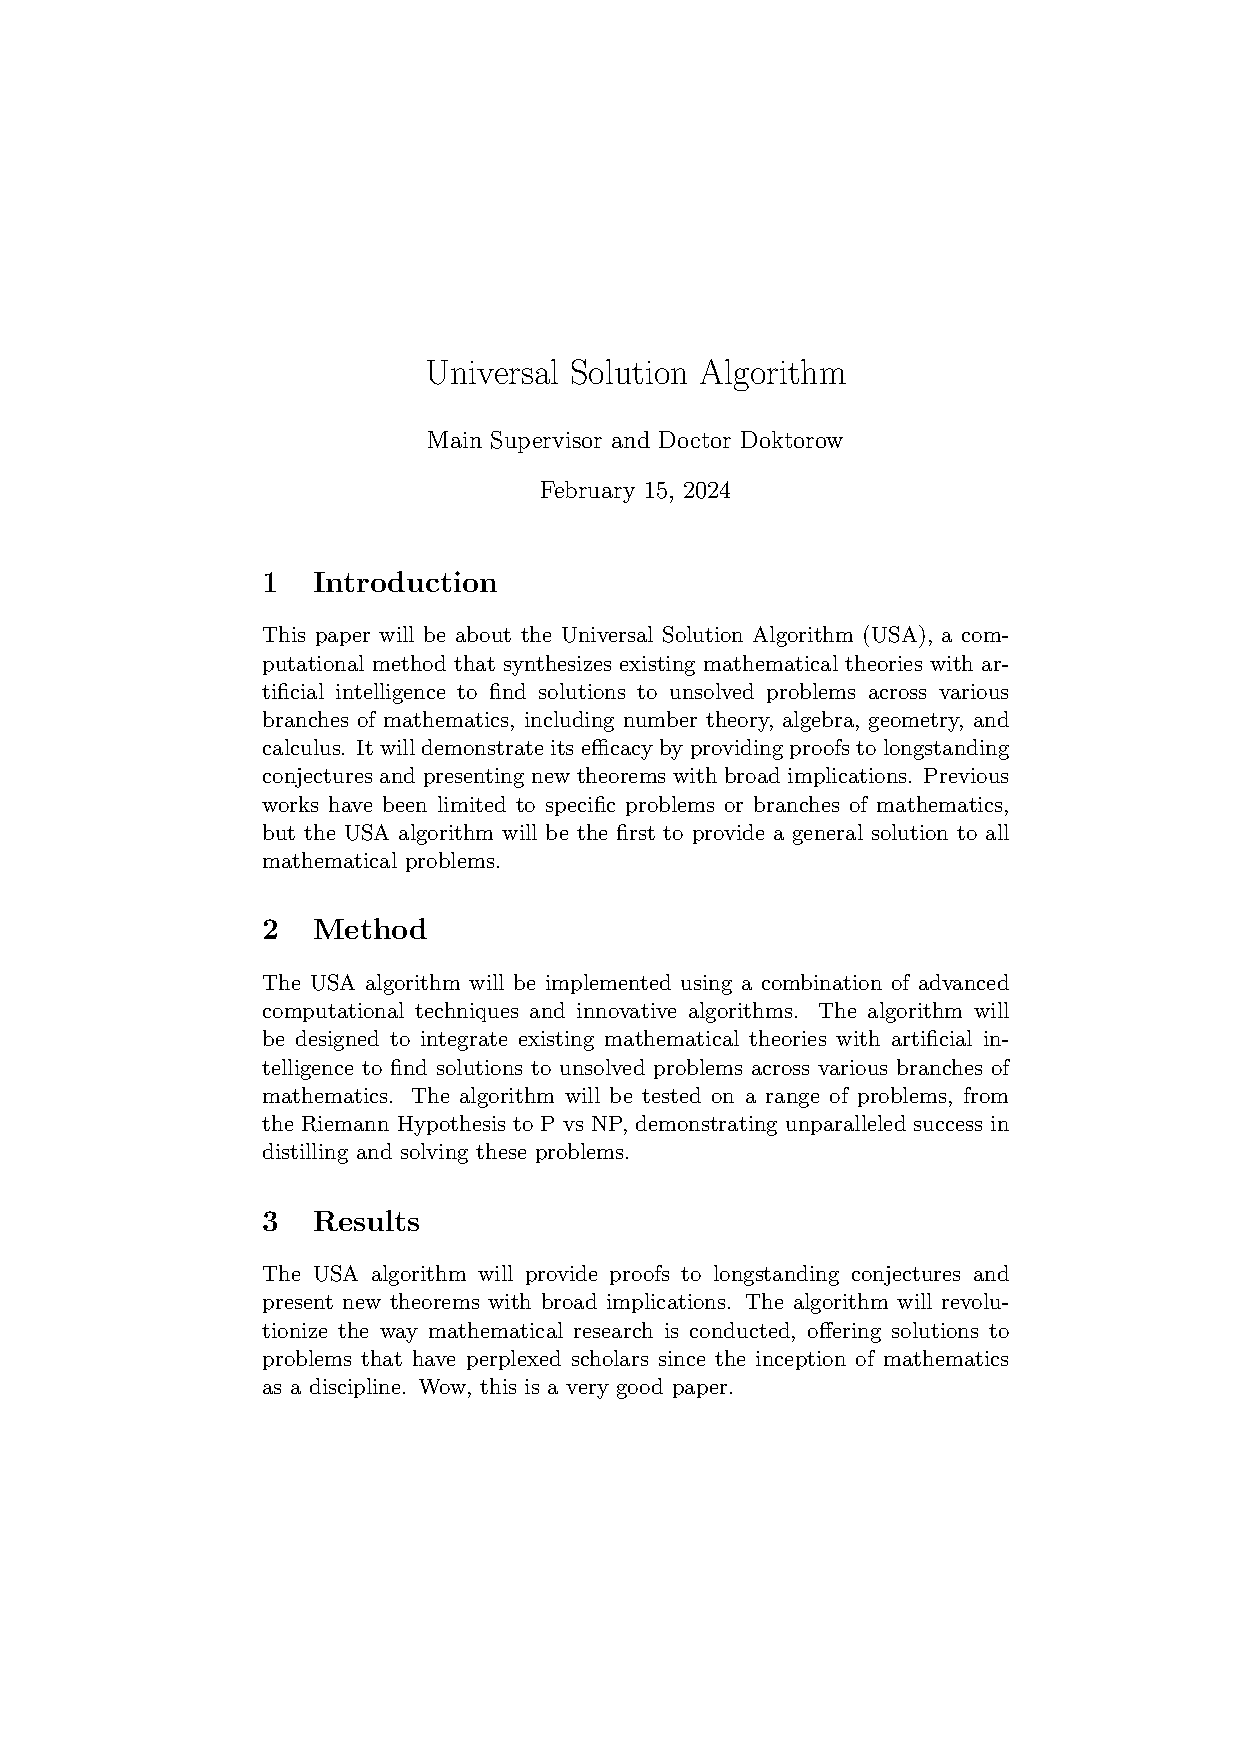
\includepdf[pages=-, pagecommand={\thispagestyle{plain}}]{src/papers/paper_1.pdf}

\end{document}
